% Outline: OUTLINE.md (course-rubric section order; Ryoo file conventions otherwise)
% Course hard rules: IEEE 2-col, each section starts a NEW PAGE, no bullets outside
% the Introduction, matplotlib-only figures, per-section page caps.
\documentclass[conference]{IEEEtran}

\usepackage[T1]{fontenc}
\usepackage[utf8]{inputenc}
\usepackage{graphicx}
\usepackage{booktabs}
\usepackage{amsmath}
\usepackage{url}
\usepackage{xcolor}
\usepackage{tikz}
\input{systems-figures.tikzstyles}
% Course rule: figure fonts AND captions >= 10 pt (IEEEtran default is 8 pt).
\usepackage[font=normalsize,labelsep=period]{caption}

% Double-column floats may only sit at a page top in standard LaTeX. With five
% of them in a nine-page paper they queue behind each other and surface pages
% after the section that discusses them. stfloats opens the page bottom as a
% second landing site, and the fractions below let a page carry more float area
% before LaTeX defers to the next one. This keeps each figure inside the
% section that argues from it, which is what the page caps are really about.
\usepackage{stfloats}
\renewcommand{\topfraction}{0.92}
\renewcommand{\bottomfraction}{0.65}
\renewcommand{\textfraction}{0.08}
\renewcommand{\floatpagefraction}{0.72}
\renewcommand{\dbltopfraction}{0.92}
\renewcommand{\dblfloatpagefraction}{0.72}
\setcounter{topnumber}{3}
\setcounter{bottomnumber}{2}
\setcounter{totalnumber}{4}
\setcounter{dbltopnumber}{3}

% Whitespace between a float and the text, tightened. IEEEtran's defaults leave
% roughly a line and a half around each; with six floats that adds up to a page
% and strands the last reference on a page of its own.
\setlength{\dbltextfloatsep}{11pt plus 2pt minus 2pt}
\setlength{\textfloatsep}{11pt plus 2pt minus 2pt}
\setlength{\floatsep}{9pt plus 2pt minus 2pt}
\setlength{\intextsep}{9pt plus 2pt minus 2pt}


\graphicspath{{figs/}}

% Two builds share these section files. The rubric build (00.tc_main_prof)
% sets this true: it moves the workload plate into Background, which is the
% one move that fixes both page violations at once -- Background reaches its
% 1.5 pages and Evaluation drops to its 3 with the minimum six figures.
\newif\ifrubric
\rubricfalse

\begin{document}

\title{Group 05: Schema-Aware Output-Length Ranking with an Abstaining
Reliability Gate for Agentic LLM Serving}

\author{\IEEEauthorblockN{Dazhi Yang, Mingye Lang, Yibo Zhang,
and Anitha Saravana Kumar}
\IEEEauthorblockA{Fairleigh Dickinson University}}

\maketitle

% Outline: Abstract (2 paragraphs, 1-2 quantitative results, 1/4 page cap).
% Ryoo craft: miniature argument; grant prior work in sentence 1, "However," pivot
% in sentence 2 reframing it as the wrong abstraction; front-load numbers.
%
% One spine: a length signal pays only where the engine leaves a queue to
% reorder. Everything else in the paper is evidence for that sentence or a
% control against it, and the abstract is ordered accordingly.
\begin{abstract}
Length-aware LLM schedulers read the prompt, or a few statistics drawn from
it. Agent traffic carries something they do not read: the JSON tool schemas a
tool-calling client attaches to every request, 18--66\% of request bytes
across the tool sets we captured from a production coding agent, naming
tools absent from the
ranker's training corpus. We fine-tune an output-length ranker on that schema
text and evaluate it in strata defined by how novel each request's tool set
is. Reading the schema is worth $+0.044$ Kendall's~$\tau$ over the same
encoder given the prompt alone (95\% paired CI $[+0.024, +0.066]$); the text
encoder as a whole is worth $+0.19$ over the tuned scalar features it
replaces, and quality holds at $\tau{=}0.64$--$0.65$ where the tool set is
partly or wholly unseen, which is where identity-based features have nothing
to look up.

A better order becomes lower latency only where the engine leaves a queue to
reorder, and that condition is set by configuration rather than by the
workload. With vLLM's running-batch cap at its default of 256 slots, mean
occupancy stayed under a fourteenth of it, the waiting queue was empty at the
90th percentile, and no ordering policy separated from another by more than
2\%. Capping the batch at sixteen puts 57--64\% of requests behind another,
and the same policies then separate: the ranker beats arrival order by 4.2\%
(0.958, 95\% CI $[0.944, 0.972]$), while ordering by prompt length, which
costs nothing to compute, runs 8.5\% slower than not reordering at all. The
signal must be paid for as well as earned --- under the gateway's own
documented 15\,ms decision timeout a third of the scores arrive too late to
use. Neither ordering nor prediction produced the largest effects we
measured: exchanging the stock scheduler cut mean time-to-last-token by 44\%
with arrival order held fixed, and prefix caching cut a further 17--23\%.
\end{abstract}

% Outline: Introduction (1 page cap; the ONLY section where bullets are allowed)
\section{Introduction}

When a coding agent talks to a language model, most of what travels
over the wire is not the user's question. Intercepting a production coding
agent (OpenCode) with an echo endpoint, we measured a single agent-loop
request. It declared 170 tools whose JSON schemas occupied 147\,kB, 67\% of
that payload, before the model read a word of the task. The share is a
range, not a constant. Within that agent's own tool set it runs 17--57\%
of request bytes (median 23.5\%), falling as conversation accumulates
around a schema block that is resent whole each turn; across every tool set
we captured the range widens to 18--66\%. Figures use
canonical serialization; raw wire bytes differ by roughly two points. No length predictor in the line we survey reads any of it.

Reading it would matter because schedulers want to know how long
each request will run. Shortest-job-first ordering needs an output-length
estimate, and a line of work has learned such estimates from prompt text
alone~\cite{fuLTR2024,tao2026ranking}. The traffic we captured violates the assumptions
behind both the scalar and the prompt-only designs. A third of its requests
carry no tools (title generation and other utility calls), each client's
schema is byte-constant across turns of the same call kind, and the tool
vocabulary in the wild is open-ended, so a learned component must handle
tools it has never seen. In our held-out
evaluation, 95.5\% of test requests carried a tool combination never seen in
training, and every tool-bearing request captured from the live agent was
composed entirely of tools foreign to the training corpus.

Our deployment context is an API gateway. Gateways are an established tier
in classical service infrastructure, where one layer owns load balancing,
admission control, caching and failure isolation, and operators now place
that same tier in front of LLM traffic with little modification. Agent
requests in this study reach the model through such a gateway (VeloxMesh),
which owns routing, admission and provider health, and which consults our
scoring service at admission time (Fig.~\ref{fig:arch}). The gateway treats
scoring as optional by design: a documented 15\,ms budget bounds the
decision, and on timeout or error the request proceeds in arrival order.
The scheduling work we survey optimizes inside the engine and does not
address this budget, so a learned predictor must fit inside it, recalibrate
it, or move off the synchronous path. This paper asks which of the gateway's
classical mechanisms remain useful for agentic LLM traffic, and whether a
learned signal can operate within the budget the gateway grants it.

We argue for two design changes. The request should be read as
\emph{text}: a ranker that consumes prompt and schema text orders unseen-tool
requests with little observed $\tau$ difference across the two adequately
powered unseen-tool strata (equivalence untested), and none of the identity
or scalar features we tested can rank tools they have never seen. Prediction
should also carry its own error bounds: our reliability gate assigns each
request a confidence measured per cold-start stratum and abstains,
preserving arrival order, wherever that measurement does not exist.

This paper contributes:
\begin{itemize}
  \item a workload characterization of live agent traffic: across captured
  tool sets, 18--66\% of
        request bytes are unread tool schema (67\% in the agent's 170-tool
        configuration), about 2\,kB per tool in its native sets,
        resent every turn; 33\% zero-tool requests; schemas byte-constant
        within a call kind;
        and a tool set entirely out of vocabulary relative to the corpus we
        train on;
  \item schema-text ranking: $+0.19$~$\tau$ over a grid-searched scalar
        baseline, with no drop detected across the two adequately powered
        unseen-tool strata (equivalence untested),
        while schema-identity
        baselines gain $+0.008$ (within noise) and \emph{lose} accuracy when
        forced to use the identity feature;
  \item a decision-budget coverage curve: neither un-truncating the schema
        nor caching its encodings makes the CPU scorer fit the documented
        15\,ms default, under which 34.6\% of decisions silently fail open;
        a timeout matched to the measured GPU scorer (50--75\,ms) restores
        98--100\% coverage, permitting that much decision latency on the
        critical path of a scored request rather than incurring it;
  \item a contention threshold for learned ordering: with the engine's
        running-batch cap at its default the queue never forms and no policy
        separates, but capping it at sixteen puts 57--64\% of requests behind
        another, and there the learned ranker beats arrival order by 4.2\%
        while ordering by prompt length runs 8.5\% slower than not reordering
        at all;
  \item a serving-level attribution: switching the scheduler implementation
        alone moved mean latency 44\% with arrival order held fixed, and
        prefix caching a further 17--23\%, in both contention regimes;
  \item an evidence-based abstaining gate: per-stratum confidences derived
        from measured ranking quality replace a hardcoded constant that
        overstates reliability by $+0.25$--$+0.46$ everywhere; the lowest
        observed ranking quality occurred on \emph{new combinations of
        familiar tools} ($n{=}78$, below our reporting threshold).
\end{itemize}

We evaluate on tool-calling corpora and on a live gateway stack
serving Qwen3.5-9B, with pre-registered criteria fixed before each
measurement. At serving time our pre-registered superiority test fails: no ordering
policy separates from another by more than 2\%, while swapping the scheduler
implementation alone cuts mean latency by 44\%. We report this attribution
result in place of the improvement we expected.

The remainder of this paper is organized as follows.
Section~II provides serving background and defines our vocabulary;
Section~III positions this work against prediction-based, prediction-free,
and imprecise-information scheduling; Section~IV details data, models, and
pre-registered criteria; Section~V presents workload characterization,
ranking, cold-start, cost, and gate results; Section~VI discusses design
consequences and limitations; Section~VII concludes.


% Outline: Background (1.5 page cap, >=2 figures; defines the paper's vocabulary)
\section{Background}

\subsection{Serving, Scheduling, and Head-of-Line Blocking}
Modern LLM engines admit requests continuously and batch them at
token granularity; continuous batching~\cite{orca2022} and vLLM's paged
KV-cache~\cite{vllm2023} are the substrate for this work. The scheduler decides which waiting request joins
the running batch next. First-come-first-served is the default, and its
weakness is classical: a long-running request admitted early delays every
short request behind it. A 2026 survey of latency in LLM agent systems
independently lists FIFO-induced head-of-line blocking among live system
bottlenecks for agentic traffic~\cite{park2026minimizing}, while placing
learned scheduling in its future-work section --- the gap this paper works in.

\subsection{Learned Output-Length Prediction}
Shortest-job-style ordering requires knowing output lengths in
advance. Since generation length is stochastic, a body of work predicts it:
S\textsuperscript{3} classifies responses into length buckets; the
learning-to-rank line~\cite{fuLTR2024} showed that \emph{relative order},
not absolute length, is what scheduling needs, training a small proxy with a
ranking loss; PARS~\cite{tao2026ranking} refined this with pairwise margin
training over a BERT encoder. All of these read the prompt (or scalar request
statistics); none consume tool-schema text.

\subsection{System Substrate: Gateway and Decision Service}
Our serving stack (Fig.~\ref{fig:arch}) fronts the engine with an
LLM gateway (VeloxMesh) that owns routing, admission, and a scheduler hook
with a documented default timeout: scoring must return within 15\,ms
(operator-configurable), after which
the gateway \emph{fails open} to arrival order. The gateway consults a
separate decision service over HTTP; that service
hosts the Ranker and applies the Reliability Gate on the gateway's behalf.
This fail-open contract is load-bearing for everything that follows: an
unreliable or slow prediction never blocks the request path.

\begin{figure*}[t]
  \centering
  % ONE grid, ONE module.
  % Columns: 0--52 | 62--114 | 124--176 -- three 52 mm columns and a single
  % 10 mm gutter. Rows: +18..-18 and -26..-62 -- two 36 mm containers and a
  % single 8 mm row gap, so every container on the page shares one top edge
  % and one bottom edge. Inside every container: 3 mm of side padding and 2 mm
  % of top and bottom padding, a header strip of one fixed 6 mm height pinned
  % top-left, and a 46x24 mm content region cut into a 9 mm body lane at
  % yc+3.5, a 6 mm connector lane, and a 9 mm body lane at yc-11.5. Every body
  % box is 46x9 mm, and every connector starts and ends exactly on the border
  % of the box it names (style: edge gap = 0).
  \begin{tikzpicture}[x=1mm,y=1mm]
    \begin{scope}[on background layer]
      \node[panel, minimum width=52mm, minimum height=36mm] (client) at (26,0) {};
      \node[panel, minimum width=52mm, minimum height=36mm] (gw)     at (88,0) {};
      \node[panel, minimum width=52mm, minimum height=36mm] (engine) at (150,0) {};
      \node[panel accent, minimum width=52mm, minimum height=36mm] (dec) at (88,-44) {};
      \node[panel, minimum width=52mm, minimum height=36mm] (verd) at (150,-44) {};
    \end{scope}

    % ---- header strips: one language, one height, one baseline per row ------
    \node[tier title, anchor=north west] at (3,16)    {Agent client};
    \node[tier title, anchor=north west] at (65,16)   {Gateway};
    \node[tier title, anchor=north west] at (127,16)  {vLLM engine};
    \node[tier title, anchor=north west] at (65,-28)  {Decision service};
    \node[tier title, anchor=north west] at (127,-28) {Verdict};

    % ---- row 1, col 1: the one captured turn every number in the paper uses --
    \node[environment component, inner sep=0pt, minimum width=46mm,
          minimum height=9mm] (cli) at (26,3.5) {OpenCode};
    \node[environment component, align=center, text width=42mm, inner sep=0pt,
          minimum width=46mm, minimum height=9mm] (turn) at (26,-11.5)
      {Captured turn\\{\sub{170 tools, 147\,kB}}};
    \draw[data flow, edge gap] (26,-1) -- (26,-7);

    % ---- row 1, col 2: gateway (one flush strip, then the scoring hook) ------
    \node[environment component, inner sep=0pt, minimum width=46mm,
          minimum height=9mm] (strip) at (88,3.5) {};
    \draw[draw=black!45, line width=.7pt] (80.333,-1) -- (80.333,8);
    \draw[draw=black!45, line width=.7pt] (95.667,-1) -- (95.667,8);
    \node at (72.667,3.5) {Admit};
    \node at (88,3.5)     {Cache};
    \node at (103.333,3.5){Route};
    \node[environment component, align=center, text width=42mm, inner sep=0pt,
          minimum width=46mm, minimum height=9mm] (hook) at (88,-11.5)
      {Scheduler hook\\{\sub{verdict due in 15\,ms}}};
    \draw[data flow, edge gap] (88,-1) -- (88,-7);

    % ---- row 1, col 3: the queue lives INSIDE vLLM, not beside it -----------
    % (verified: the gateway attaches the verdict to the forwarded request,
    %  VeloxMesh internal/ltr/decision.go:218; the policy reads it back from
    %  the request's extra_args inside the engine, vllm_scheduler.py:87)
    \node[proposed component, align=center, text width=42mm, inner sep=0pt,
          minimum width=46mm, minimum height=9mm] (sched) at (150,3.5)
      {Scheduler\\{\sub{reorders trusted slots}}};
    \node[trusted slot, minimum width=10mm, minimum height=9mm] (q1) at (132,-11.5) {};
    \node[pinned slot,  minimum width=10mm, minimum height=9mm] (q2) at (144,-11.5) {};
    \node[trusted slot, minimum width=10mm, minimum height=9mm] (q3) at (156,-11.5) {};
    \node[pinned slot,  minimum width=10mm, minimum height=9mm] (q4) at (168,-11.5) {};
    % Both ends land on a slot's top border; the swap needs no chip because the
    % scheduler box above it already says what the swap is.
    \draw[data flow, edge gap]
      (156,-7) .. controls (150,-2) and (138,-2) .. (132,-7);

    % ---- row 2, col 2: decision service, one flush three-lane stack ---------
    \node[proposed component, inner sep=0pt, minimum width=46mm,
          minimum height=24mm] (stack) at (88,-48) {};
    \draw[draw=sysaccent!85!black, line width=.9pt] (65,-45) -- (111,-45);
    \draw[draw=sysaccent!85!black, line width=.9pt] (65,-51) -- (111,-51);
    \node at (88,-40.5) {Stratum classifier};
    \node at (88,-48) {Reliability Gate};
    \node at (88,-55.5) {Schema-aware Ranker};

    % ---- row 2, col 3: the verdict, as two boxes an arrow can land on -------
    \node[environment component, align=center, text width=42mm, inner sep=0pt,
          minimum width=46mm, minimum height=9mm] (fo) at (150,-40.5)
      {Arrival order\\{\sub{abstain, or 15\,ms passes}}};
    \node[proposed component, align=center, text width=42mm, inner sep=0pt,
          minimum width=46mm, minimum height=9mm] (key) at (150,-55.5)
      {Reorder key\\{\sub{trusted: S3 / S4}}};
    \draw[degraded flow, edge gap, lane turn]
      (111,-48) -- (119,-48) -- (119,-40.5) -- (127,-40.5);
    \draw[data flow, edge gap] (111,-55.5) -- (127,-55.5);

    % ---- the two inter-row connectors: ask down, verdict up ----------------
    % Each chip sits beside its own arrow, and the arrow is offset by half the
    % chip so that arrow+chip centre on the column axis (x=88 and x=150).
    \draw[data flow, edge gap] (75.75,-18) -- (75.75,-26);
    \node[metric badge, anchor=west] at (77.25,-22) {score, 15\,ms};
    \draw[data flow, edge gap] (141.75,-26) -- (141.75,-18);
    \node[metric badge, anchor=west] at (143.25,-22) {verdict};

    % ---- edges on the serving path -----------------------------------------
    \draw[data flow, edge gap, lane turn] (49,-11.5) -- (57,-11.5) -- (57,3.5) -- (65,3.5);
    \draw[data flow, edge gap] (111,3.5) -- (127,3.5);

    % ---- legend: a compact band, deliberately smaller than a subsystem ------
    \node[tier band, minimum width=52mm, minimum height=16mm, inner sep=0pt]
      at (26,-44) {};
    \node[proposed component, inner sep=0pt, minimum width=7mm,
          minimum height=4.4mm] at (8.5,-39) {};
    \node[fact label, fill=none, anchor=west, text=black!75] at (13.5,-39)
      {added by this work};
    \node[environment component, inner sep=0pt, minimum width=7mm,
          minimum height=4.4mm] at (8.5,-44) {};
    \node[fact label, fill=none, anchor=west, text=black!75] at (13.5,-44)
      {unchanged substrate};
    \draw[degraded flow] (5,-49) -- (12,-49);
    \node[fact label, fill=none, anchor=west, text=black!75] at (13.5,-49)
      {fail-open path};
  \end{tikzpicture}
  \caption{The gateway scores at admission inside a 15\,ms budget and
  forwards the verdict; the engine's scheduler reorders trusted slots among
  themselves and leaves abstained ones where they arrived. A timeout or an
  abstention yields arrival order.}
  \label{fig:arch}
\end{figure*}

\begin{figure*}[t]\centering
  % Source: runs/coldstart/ (999 test requests, 3 seeds) and the gate's
  % validation fit; every number is read from those artifacts at build time.
  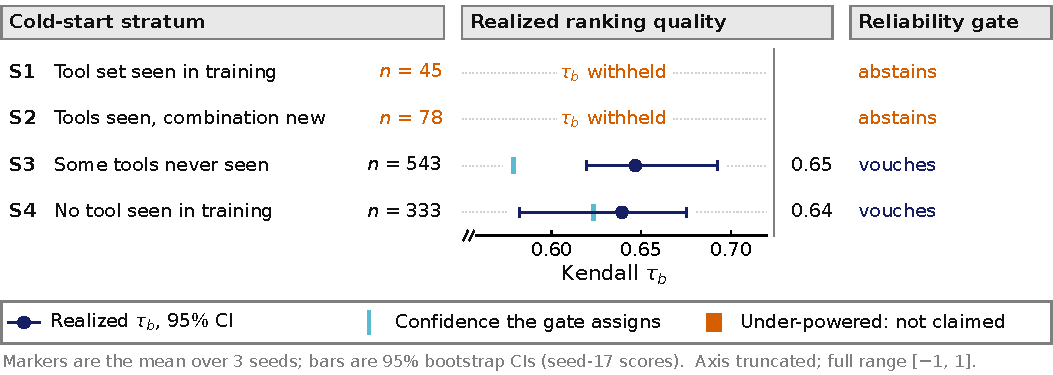
\includegraphics[width=\linewidth]{strata.pdf}
  \caption{The four cold-start strata, and which of them the paper is
  allowed to speak for. S1 and S2 hold too few test requests to support a
  claim, so their Ranking Tau is withheld and the gate routes them to
  Fallback.}
  \label{fig:strata}
\end{figure*}

\subsection{Vocabulary}
Throughout, the \emph{Ranker} is the fine-tuned BERT model scoring a
request's expected output length; the \emph{Reliability Gate} is the runtime
decision of whether that score may influence queue order; \emph{Fallback}
means serving in arrival order because the gate withheld trust.
\emph{Ranking Tau} is Kendall's $\tau_b$~\cite{kendall1938} between predicted and true
output-length order on held-out data. \emph{Cold-Start Transfer} measures
Ranking Tau on test strata whose tool sets were unseen in training, within
the same workload family: S1 (seen combination), S2 (new combination of seen
tools), S3 (partially new tools), S4 (all-new tools); Fig.~\ref{fig:strata}
gives each stratum's size and what the gate does with it. It is distinct from
\emph{Cross-Workload Transfer}, which changes the workload family entirely.

% Outline: Related Work (1 page cap). Ryoo craft: pure gap-framing, never survey;
% batch-cites to establish each field; bold run-in headers; differentiate by AXIS;
% first-person "Our work ..." differentiators; concede-then-pivot, never dismiss.
\section{Related Work}

\subsection{Learned Length Prediction for Scheduling}
A substantial line learns output-length signals to approximate
shortest-job-first serving~\cite{ssjf2024,fuLTR2024,tao2026ranking,elis2025},
progressing from length-bucket classification to relative-rank training, the
insight we inherit: scheduling needs \emph{order}, not absolute
length~\cite{fuLTR2024}. PARS, now peer-reviewed at ISC High Performance
2026, pairs a BERT encoder with pairwise margin training and demonstrates
cross-model robustness~\cite{tao2026ranking}. However, every predictor in
this line reads the prompt or scalar request statistics; none consumes
tool-schema text, and none is evaluated on requests whose tools were absent
from training. Our work fills this gap: schema text as
predictor input, and a novelty-stratified evaluation in which 95.5\% of test
requests carry tool combinations unseen in training --- the regime our
single-client live capture exhibits throughout.

\subsection{Prediction-Free Scheduling}
A newer position holds that tail latency does not need prediction at all.
UniBoost's distribution-aware boosting beats even an \emph{oracle}-length
SRPT baseline by 35.1\% on P99 time-to-last-token in its Table~2
configuration~\cite{beyondPrediction2026}, and starvation-free preemptive
designs make adjacent arguments~\cite{fastServe2026,tie2026}. We
therefore make no tail claims: if an oracle loses on P99, better ranking
accuracy will not repair that, so our endpoints are means and goodput. The concession is scoped by the papers' own designs, however:
UniBoost evaluates no tool-calling workload, disables prefix caching for
experimental control, and is prediction-free but not feature-free --- its
scheduler consumes prompt length, the same class of signal our weakest
baseline uses. Whether its result transfers to agentic traffic is, by its
own construction, open.

\subsection{Scheduling Under Imprecise Information}
JITServe is the strongest published treatment of acting on unreliable
estimates: quantile-forest \emph{upper bounds} on length, refined every
$\sim$50 generated tokens, drive grouped goodput scheduling within 3--9\% of
an oracle on a 16-GPU cluster --- with BERT-class predictors explicitly
rejected at 56--187\,ms under load against a forest costing 11--24\,ms at
those same loads (its oft-quoted 7\,ms is the lightest, 8-requests/s
point)~\cite{jitServe2026}. Its tool awareness is structural: tools enter as
identity and duration in a dependency graph, never as text into the length
model. We position our gate as complementary, not competitive. JITServe
absorbs uncertainty by always scheduling against a pessimistic bound; our
gate \emph{detects} where trust has no measured basis and abstains,
preserving arrival order --- the ``explicit fallback policies'' its authors
name as an open problem under distribution shift. Agent-serving systems that
exploit workflow structure~\cite{agentix2026,infercept2024} are orthogonal:
they schedule around tool-call \emph{interruptions}, not around length
uncertainty.

\subsection{Schemas as Model Input; Unseen-Tool Evaluation}
Fine-tuning small encoders on schema text is established practice in tool
learning --- it is how function-calling models are
trained~\cite{toolace2024,qin2024toolllm,patil2024gorilla} --- and
Switchcraft packs function signatures into a DistilBERT to route requests
across models by predicted \emph{correctness}~\cite{switchcraft2026}. The
distinction we claim is therefore narrow and specific: schema text
$\rightarrow$ output-length rank $\rightarrow$ queue order is, to our
knowledge, unoccupied; Switchcraft itself lists benchmark-shift
quantification as future work; our Cold-Start Transfer strata measure that
axis. For the stratified design we follow tool-learning precedent:
ToolLLM evaluates at unseen-instruction, unseen-tool, and unseen-category
levels~\cite{qin2024toolllm}, licensing our S1--S4 \emph{design} though not
our metric (it scores task success, not length rank). BFCL's crowd-sourced
split targets contamination control, a different axis~\cite{patil2025bfcl},
and Gorilla's holdout is random --- its ``zero-shot'' denotes retriever
absence, not unseen APIs~\cite{patil2024gorilla} --- so neither substitutes
for tool-novelty stratification.

\subsection{The Serving Substrate: Gateways, Admission, Prefix Reuse}
Our contribution sits between two systems layers that are usually studied
separately. Below the engine, continuous
batching~\cite{orca2022} and paged attention~\cite{vllm2023} set the
execution substrate, and prefix reuse --- RadixAttention in
SGLang~\cite{sglang2024} and the prefix caching now standard in
vLLM --- exploits the repetition our capture exhibits, a
schema resent byte-identically on every turn of a given call kind; our
ordering runs hold it
disabled to isolate ordering, and one round enables it to measure it. Above the engine, gateways
own admission: overload control in production RPC systems sheds load
by priority when queues exceed bounds~\cite{dagor2018}, and the
gateway we deploy on implements the same pattern as queue guards with
priority bypass. Admission decides \emph{whether and when} a request
reaches the engine; the engine's scheduler decides \emph{which}
waiting request runs next. Our predictor feeds the second decision,
and its budget is set by the first, so a scoring path
slower than the configured admission timeout is excluded regardless of
its ranking accuracy; the timeout itself is an operator choice.


% Outline: Methodology (1 page cap, >=2 tables; recipes + provenance, no results)
\section{Methodology}

\subsection{Data and Labels}
Training and offline evaluation use a 6{,}000-request stratified
sample of ToolACE tool-calling conversations, labeled with completion
lengths measured against Qwen3.5-9B under frozen generation controls
(temperature 0, top-p 1, seed 42, max 4096 tokens). We chose Qwen3.5-9B
because it is open-weight, carries first-class tool-calling support in vLLM
(native tool-call and reasoning parsers), and at 9B serves in bf16 on a
single 48\,GB card with 16k context. Using the same model for labeling and
serving keeps the label distribution matched to the engine under test. Three rows whose labeling
runs failed are declared as structural exclusions rather than silently
dropped, and three censored rows are excluded, leaving 5{,}994 eligible rows
split 3{,}997/998/999 by a per-row split column
fixed before any experiment; every run in this paper shares that split.
Label censoring is 0.05\%.

\subsection{Ranker and Feature Variants}
The Ranker is BERT-base~\cite{bert} producing a scalar score
$s_\theta(x) \in [0,1]$ from input rendered as
\texttt{[USER]}\,prompt\,\texttt{[TOOLS]}\,schema, truncated at 512 tokens.
We fine-tune with the pairwise margin objective
\begin{equation}
\mathcal{L}(x_a, x_b) = \max\bigl(0,\; -y \cdot (s_\theta(x_a) - s_\theta(x_b)) + m\bigr),
\end{equation}
where $y = \pm 1$ encodes which request produced the longer completion,
$m{=}1.0$, and pairs enter training only when their normalized length gap
exceeds $\delta{=}0.2$; three seeds (17/42/73) vary initialization and pair
shuffling over one fixed split. Table~\ref{tab:variants} lists the Feature Variants; the
full-context arm is reported void because the same 512-token cap leaves
80\% of its inputs truncated --- a disclosure, not a result.

\begin{table}[t]
  \caption{Feature variants and offline recipe. All variants share one fixed
  3{,}997/998/999 split of the labelled ToolACE sample.}
  \label{tab:variants}
  \centering\footnotesize
  \setlength{\tabcolsep}{3.5pt}
  \begin{tabular}{@{}lll@{}}
    \toprule
    Variant & Ranker input & Note \\
    \midrule
    prompt\_only & prompt text & encoder-strength control \\
    prompt\_schema & prompt + schema text & the proposed input \\
    full\_context & + history & void under truncation \\
    \midrule
    scalar (LightGBM) & 5 request statistics & fixed + 20-config grid \\
    identity (hash) & scalar + tool-set fingerprint & lookup emulation \\
    \bottomrule
  \end{tabular}
\end{table}

\subsection{Baselines and Identity Features}
The scalar baseline is LightGBM~\cite{lightgbm} over prompt length (chars,
words),
schema length, tool count, and history turns --- the scalar family
gateway-side length predictors describe --- in a fixed-hyperparameter form and a 20-configuration
grid search whose configuration is chosen on the validation split, never on
test; the stronger result is the baseline of record. The recipe is
deterministic with respect to seed (no stochastic sampling consumes the
random state), verified by bit-exact rerun. Identity baselines fingerprint
the tool set as SHA-256 over sorted tool names --- never over the raw schema
string, which embeds per-request timestamps that would fake uniqueness ---
and add out-of-fold per-fingerprint label statistics, emulating a deployed
per-client lookup table with a global-mean fallback for unseen keys.

\subsection{Cold-Start Strata and the Gate}
The fixed test split is partitioned into S1--S4 by fingerprint and
tool-name novelty against the training vocabulary. Strata under 100 rows
(S1$=$45, S2$=$78 at test) are withheld from headline claims; they may
inform design when disclosed with their size. The abstention set itself is
fixed on the validation split alone: S1 and S2 fall below the same 100-row
floor there ($n{=}74$ and $n{=}82$, against 472 and 370 for S3 and S4), so
the gate has no validation basis on which to vouch for them. Their test
sizes are reported for power, never used to set the rule. The Reliability Gate assigns each stratum the
lower bound of the 95\% session-clustered bootstrap~\cite{efron1979}
confidence interval of
\emph{validation} Ranking Tau --- fit on validation, evaluated on test ---
and abstains (confidence 0) on strata it cannot measure, including zero-tool
requests:
\begin{equation}
c(x) = \begin{cases}
  \max\bigl(0,\ \underline{\tau}_{95}(S(x))\bigr) & S(x) \in \{\mathrm{S3},\mathrm{S4}\} \\
  0 & \text{otherwise,}
\end{cases}
\end{equation}
where $S(x)$ is the request's stratum under the training vocabulary and
$\underline{\tau}_{95}$ the lower bootstrap bound of validation Ranking Tau.
A request is trusted when $c(x) \ge 0.5$; abstained requests keep their
arrival slots, and trusted requests reorder only among trusted slots. This confidence is a stratum-level abstention score, not a
calibrated probability.

\subsection{Serving Configuration}
The gateway runs in its default configuration plus exactly six
environment variables: listen address, API key, upstream provider and
model, the decision endpoint, and its timeout. Its request-shaping
pipeline, provider combos, semantic cache and scheduler-side queue
limits are all at their disabled defaults. The decision timeout is
6{,}000\,ms during ordering runs --- deliberately far above the
documented 15\,ms scheduling budget, so that fail-open never fires;
differences between ranked and unranked arms then bundle the ranking
signal with the synchronous scoring cost that carries it, and are read
as such. The budget itself is enforced and measured in dedicated arms
at 15\,ms (the documented default), 50 and 75\,ms
($\approx$1.3$\times$ and 2$\times$ the Ranker's GPU median), tracing
in-budget coverage against the operating point an operator who had
measured our scorer would actually set. vLLM prefix caching is disabled uniformly across the default-cap
ordering arms, verified from the engine's reported hit rate rather
than from the flag alone. It is enabled in the arm that measures its
effect and in all four arms of the capped-batch round, where holding it
on everywhere means it cannot separate them.

\subsection{Serving Environments and Provenance}
Table~\ref{tab:envs} pins both environments. Serving experiments
run on a single cloud RTX~4090 with 48\,GB VRAM (a vendor-modified memory
configuration common on Chinese GPU clouds); the decision service runs the
Ranker in fp16 with micro-batching (batch $\le$ 8, 3\,ms window) and a
reliability threshold of exactly 0.5. All vLLM capacity and cache settings
are held constant across every arm of every comparison; prefix caching is
disabled in every default-cap ordering arm --- verified from the engine's own
reported hit rate rather than from the flag alone --- and enabled in the
round that measures it and throughout the capped-batch round. The scheduler is
replaced through vLLM's~\cite{vllm2023} \texttt{--scheduler-cls} seam. Each
policy arm subclasses the engine's scheduler and re-sorts only the waiting
queue before each step, all else stock code; the stock pair differs in
scheduler implementation as well, the difference E5's attribution control
measures.

\begin{table}[t]
  \caption{Environment provenance for the two measurement platforms, which
  are separate rentals: labelling and fine-tuning ran first, serving weeks
  later.}
  \label{tab:envs}
  \centering\footnotesize
  \setlength{\tabcolsep}{3.5pt}
  \begin{tabular}{@{}lll@{}}
    \toprule
     & Training & Serving \\
    \midrule
    GPU & RTX 3090 24\,GB & RTX 4090 48\,GB (modified) \\
    Driver / CUDA & --- & 580.159.03 / 13.0 wheels \\
    Engine & vLLM 0.19.1, torch 2.10 & vLLM 0.24, torch 2.11 \\
    Model & Qwen3.5-9B (labels) & Qwen3.5-9B, bf16 \\
    Scheduler seam & --- & \texttt{--scheduler-cls} per arm \\
    \bottomrule
  \end{tabular}
\end{table}

% Outline: Evaluation (3 page cap, >=6 figures; narrative order = story acts)
% Numbers of record: SYNC-CHECKLIST-2026-07-26.md; claims->evidence map in outline.md.
% Figure inventory for the >=6 rule, at exactly six: fig:workload, fig:tau,
% fig:overhead, fig:gate, fig:regime, fig:block1. The cold-start plate was
% dropped to reach the 3-page budget; its numbers are all in the prose and
% Fig. 2 in Background carries the per-stratum view.
\section{Evaluation}
\label{sec:eval}

\subsection{E1: What Agent Requests Are Made Of}
Fig.~\ref{fig:workload} characterizes the capture. It covers 75 requests
across 25 tasks of a production coding agent.
Each tool in the native sets contributes about 2\,kB of schema
(1.8--2.1\,kB), giving 21\,kB for ten native tools; the denser 170-tool
configuration totals 147\,kB, resent whole every turn. That fixed per-turn
cost is an unstable share of the request: 17\% to 57\% within the native
configuration alone (median 23.5\%), and 67.0\% with 170 tools. Within a
call kind the tool set is byte-identical across turns, and the 75 requests
carry only three distinct sets. Against the ToolACE vocabulary, every
tool-bearing live request classified as S4.
\ifrubric\else
\begin{figure*}[t]\centering
  % Source: probes/agent-traces-2026-07-26/MANIFEST.md + schema-variability probe.
  
\includegraphics[width=\linewidth]{workload.pdf}
  \caption{Captured agent traffic: across the captured tool sets schemas are
  18--66\% of request bytes, a
  third of requests carry no tools, and completion medians split 6 versus 58
  tokens, so the pooled median of 42 describes neither kind.}
  \label{fig:workload}
\end{figure*}
\fi

\subsection{E2: Schema Text vs.\ Scalars vs.\ Identity}
Fig.~\ref{fig:tau} gives the headline offline result. Reading the request as
text beats the scalar baseline family by $+0.19$~$\tau$ against the tuned
baseline of record (0.6302 vs.\ 0.4395; fixed form 0.4268). The prompt-only
control reaches 0.5865, so roughly 77\% of that gap comes from the text
encoder and 23\% from the schema text. Isolated, the schema is worth
$\Delta\tau_b = +0.0437$ (95\% session-clustered paired CI
$[+0.024, +0.066]$). Schema identity is nearly worthless: a
fingerprint-plus-lookup baseline gains $+0.008$, inside its own $\pm 0.035$
interval, because only 4.5\% of test requests share a fingerprint with
training.

\begin{figure}[tb]\centering
  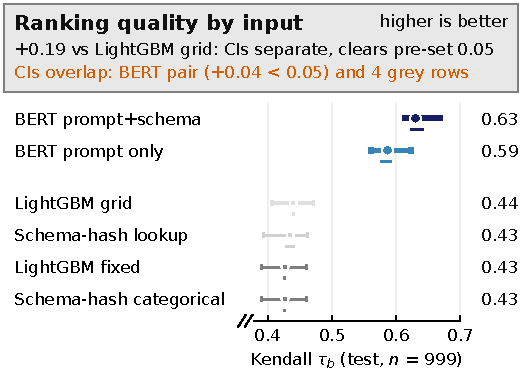
\includegraphics[width=\linewidth]{ranking.pdf}
  \caption{Ranking quality by input family: prompt-plus-schema text exceeds
  the tuned scalar baseline by $\Delta\tau_b{=}+0.191$. Dots are the mean
  over 3 seeds; capped bars the 95\% bootstrap CI on seed 17 alone; the lane
  below each row the min--max across seeds, a tick where that spread is
  zero.}
  \label{fig:tau}
\end{figure}

The same models are evaluated on the two strata Fig.~\ref{fig:strata} clears
for use: S3 (partially new tools, $n{=}543$) and S4 (all-new tools,
$n{=}333$). Both
pre-registered criteria pass on both strata against the tuned baseline, and
schema-text $\tau$ differs by only 0.0075 between them (0.647 and 0.639,
against 0.630 overall). We ran no equivalence test, so this is consistent
with no degradation rather than a demonstration of it. What does not hold
flat is the \emph{margin}: schema text leads the tuned baseline by $+0.25$
on S3 but only $+0.14$ on S4, because the scalar baseline itself scores
higher where no tool is familiar ($\tau_b$ 0.50 against 0.40). Reading the
schema keeps its own quality on wholly unseen tools; it does not widen its
lead there.

\subsection{E3: Deployment Cost and Two Failed Rescues}
Fig.~\ref{fig:overhead} prices the admission path the scorer sits on.
The Ranker costs 722\,ms at p99 on production CPU settings at the deployed
concurrency of eight, 48$\times$ the gateway's 15\,ms contract and still
8$\times$ over it served serially. Two pre-registered rescues fail.
\emph{Un-truncation}: 71\% of schemas exceed the 512-token cap, yet a
two-tower encoder reading the whole schema moves $\tau$ by $+0.0008$ (S3)
and $-0.0112$ (S4), intervals overlapping. \emph{Caching}: precomputing the
schema tower yields $1.9\times$, still 25$\times$ over contract at
concurrency 8 (4.3$\times$ serial). On the serving GPU with fp16
micro-batching, scoring costs 37.9\,ms at p50, $6.0\times$ faster than
unbatched GPU inference and
$16.6\times$ faster than the CPU path at the same percentile (628.8\,ms
p50). Enforcing a budget end to end is a different measurement, and we
report it over every request the gateway handled rather than over the scored
subset: under the documented 15\,ms default, 801 of 2{,}315 requests
(34.6\%) fail open into arrival order, silently; at 50\,ms that falls to
2.0\% and at 75\,ms to zero. The denominator includes requests the gate
never scores at all --- the zero-tool third of the traffic and the strata it
abstains on --- so 34.6\% is the share of \emph{traffic} left unordered, not
the share of scoring attempts that miss the budget, which is necessarily
larger.
\begin{figure*}[tb]\centering
  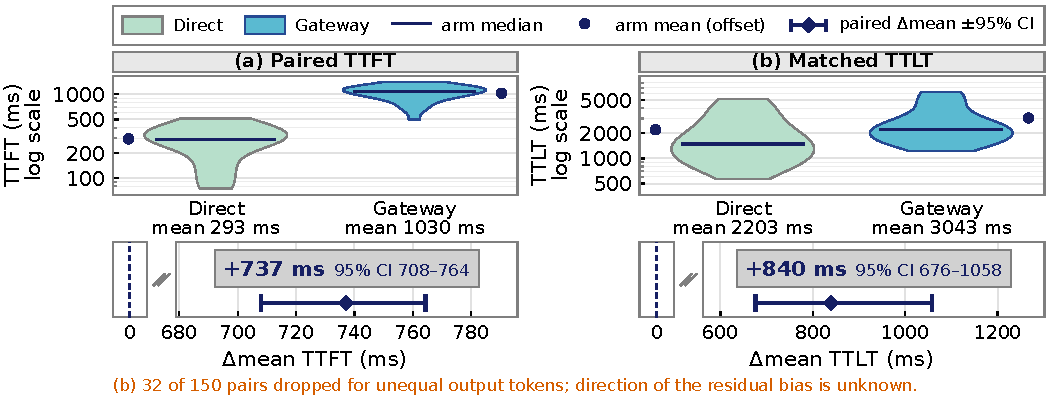
\includegraphics[width=\linewidth]{overhead.pdf}
  \caption{Admission-time scoring versus direct: $+$737\,ms TTFT and
  $+$840\,ms TTLT over the whole added path. Panel (a) is 150 paired
  requests and (b) the 118 of them with equal output tokens; violin bodies
  and $y$-axes are trimmed to p5--p95 of each arm, and intervals are
  2{,}000$\times$ bootstrap percentile CIs.}
  \label{fig:overhead}
\end{figure*}

\subsection{E4: Assigned versus Realized Confidence}
Fig.~\ref{fig:gate} contrasts the confidence each rule assigns with the
ranking quality it actually delivered.
The placeholder constant confidence (0.9) overstates realized ranking
quality on every stratum, by $+0.25$ to $+0.46$; the lower CI bound of
validation $\tau$ per stratum, abstaining where it cannot be measured, did
not overstate on any stratum here: its closest approach to overstating was
$-0.016$ on S4, and its largest understatement $-0.068$ on S3. S2 is where
the Ranker fails: familiar tools in new combinations realize $\tau = 0.44$,
against 0.60 on S1, 0.65 on S3 and 0.64 on S4 --- 0.16 to 0.21 below every
other stratum. At $n{=}78$ that sits below our reporting threshold, so we
read it as a design signal rather than a result, which is why
Fig.~\ref{fig:strata} plots neither it nor S1's.
\begin{figure*}[tb]\centering
  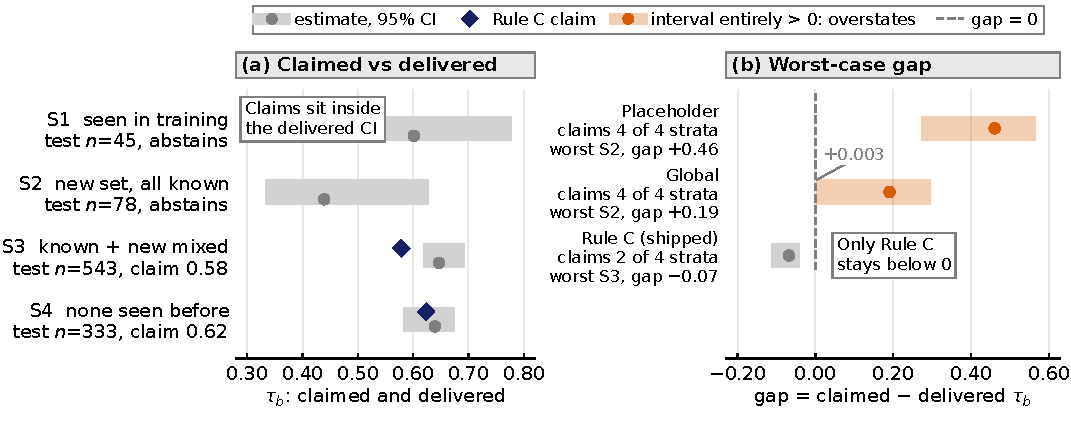
\includegraphics[width=\linewidth]{gate.pdf}
  \caption{Assigned versus realized confidence: the placeholder constant
  overstates on every stratum; Rule~C did not on this split, at the cost of
  abstaining where it cannot measure.}
  \label{fig:gate}
\end{figure*}

\subsection{E5: Serving-Level Scheduling}
We replayed 2{,}075 requests open-loop at 3.96 requests/s, 90\% of the
highest rate the stock scheduler sustained under a 95\% completion criterion
(4.4\,requests/s). Six schedulers share one arrival schedule: stock
first-come-first-served, a shim wrapping it unchanged, and four on our own
base, \emph{PolicyFCFS} (arrival order, no scorer), \emph{PromptLengthSJF}
(prompt length), \emph{PureLTR} (Ranker score) and \emph{GatedRuleC} (Ranker
score where the gate vouches). The pre-registered endpoint is pooled mean
time-to-last-token (TTLT), compared as paired-mean ratios with hierarchical
bootstrap intervals against a pre-declared 3\% margin; time-to-first-token
(TTFT) is reported only where the admission path is priced.

The attribution control comes first (Fig.~\ref{fig:block1}).
\emph{PolicyFCFS} and stock serve the same requests in the same arrival
order and differ only in scheduler implementation; PolicyFCFS records a
paired mean-TTLT ratio of $0.560$ ($[0.540, 0.581]$), so that 44\% reduction
arrives with the switch of implementation itself, none of it contributed by
ordering. Interposition does not explain it: the shim lands within 2\,ms of
stock (4903 vs.\ 4905\,ms). What does differ is the base class: the policy
arms subclass vLLM's \texttt{AsyncScheduler}, which overlaps scheduling with
model execution, while stock and the shim run the synchronous one --- the
likeliest mechanism, though the one-line ablation confirming it did not make
our budget.

Against the same-base control, ordering does not move the endpoint here. The
superiority test fails: GatedRuleC versus PromptLengthSJF gives $1.008$
($[0.979, 1.041]$), an interval containing one. Safety passes: against
PolicyFCFS the ratio is $0.996$ ($[0.970, 1.023]$), inside the 3\% margin,
and with an empty queue the gate itself costs at most 1.4\% (GatedRuleC against
PureLTR, $1.003$, $[0.991, 1.014]$; Sec.~V-F).

The order logs quantify how often ordering could act and show that the
policies acted when able. Across 77{,}000 scheduling steps per arm the
waiting queue was empty at p90 and held two waiting requests in under 1\% of
steps; 11.9--12.5\% of requests first entered a queue of depth two or more.
Expressing an order needs two requests that were \emph{already} waiting to
meet in the same step. That happened in 293--324 steps per arm, and the
policies rewrote 262--307 of them (87--95\%), while \emph{PolicyFCFS}
rewrote none. Ordering was executed on nearly every opportunity it had and
mean TTLT did not move. This round did not isolate why: three mechanisms are
consistent with it, the replay's compressed job-size variance, a two-deep
queue where a swap moves a request by at most one slot, and residual ranking
error at $\tau{=}0.63$. Round~A separates none of them; E6 does.

A second round replays all six arms with vLLM prefix caching enabled and
nothing else changed. The stock arms bridge the sessions, their on/off
ratios agreeing to four decimal places (0.8291 vs.\ 0.8290), and the
engine's log confirms the cache took effect (62.1\% peak hit rate). Caching
cuts pooled mean TTLT by 17.1\% on the stock pair and 22--23\% on the four
policy-base arms. The policy intervals overlap the bridge's, so the larger
gain is suggested rather than established, and the experiment did not
isolate the schema's share of it.

A third round at 6.4\,requests/s in three blocks of cold engine launches
fails the same check (exposure only 14.3--15.0\%, \emph{not one} carry-over
step across twelve launches), so it is non-diagnostic for superiority. On
those independent launches GatedRuleC gives $1.001$ ($[0.988, 1.015]$),
$1.006$ ($[0.993, 1.020]$) and $1.006$ ($[0.995, 1.018]$) against
PromptLengthSJF, PolicyFCFS and PureLTR, all inside the 3\% margin.

\subsection{E6: Ordering Under Contention}
None of those rounds formed a queue: the running-batch cap sat at vLLM's
default of 256 slots while only eleven to nineteen requests were in flight.
E6 caps it at 16 and repeats the question at 6.4 requests/s with prefix
caching on and one cold launch per arm. Three conditions therefore differ
from round~A besides the cap --- rate, caching and launch structure --- so
the comparison across panels is between regimes rather than between two
otherwise identical runs; what is held exactly is the workload, the arrival
offsets, the checkpoint, and the four policies being contrasted, which is
what makes the ordering comparison \emph{within} each regime clean. The cap
is an instrument, not a recommendation. A scheduler can only act where
requests wait, and what we could vary at our budget was the number of slots
rather than the arrival rate needed to fill 256 of them; a deployment
reaches the same condition whenever offered concurrency exceeds the slots
it has, whether because the cap is low or because long contexts exhaust the
KV cache first. What E6 tests is therefore the regime, not the number: the
claim is that ordering pays once a queue exists, and the cap is how we made
one. The
manipulation check passes this time: 57.5--63.6\% of requests entered a
queue of depth two or more, p90 depth reached 8 to 14, and 5{,}914 to
7{,}121 steps per arm carried two requests that had both waited earlier,
against 293--324 in round~A. The policies rewrote 1{,}817 to 6{,}607 of
them, and \emph{PolicyFCFS} again rewrote none.

Ordering now moves the endpoint (Fig.~\ref{fig:regime}), and the
pre-registered primary test passes for the first time: GatedRuleC versus PromptLengthSJF gives $0.966$
($[0.935, 0.998]$), an upper bound below one. What pays is the learned
signal. PureLTR beats arrival order by 4.2\% ($0.958$, $[0.944, 0.972]$),
while the free length heuristic runs 8.5\% \emph{worse} than doing nothing
($1.085$, $[1.051, 1.122]$), so rendered prompt length is a poor proxy for
output length; over 2{,}025 shared sessions pooled mean TTLT is 2.797\,s for
PureLTR against 3.169\,s for PromptLengthSJF. The two regimes also separate
the gate's cost:
GatedRuleC against PureLTR was $1.003$ ($[0.991, 1.014]$) with an empty
queue and is $1.095$ ($[1.079, 1.112]$) here, and against PolicyFCFS it is
$1.049$ ($[1.033, 1.065]$), outside the 3\% margin. Abstention pins S1, S2
and zero-tool requests in their arrival slots, and once the queue is deep
those pinned requests block the ones behind them. Abstaining is free when
nothing is waiting and costly when something is.

\begin{figure*}[tb]\centering
  % Source: runs/block1-main/matrix (default cap) and
  % runs/capped-batch/matrix (cap 16); same workload, same arrival offsets,
  % same checkpoint. Ratios and intervals are the paired bootstrap.
  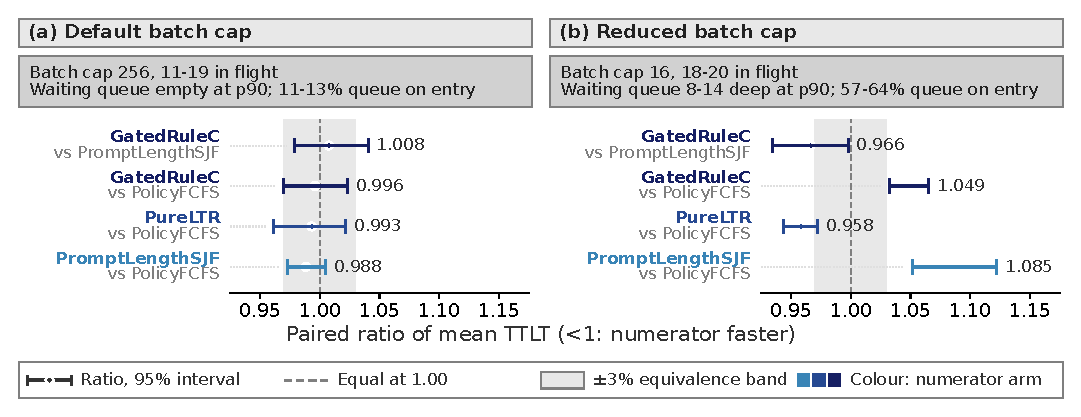
\includegraphics[width=\linewidth]{regime.pdf}
  \caption{One engine setting decides the paper's answer: the same four
  policies on the same workload, with the default running-batch cap no pair
  separates, and with the cap reduced every pair does. Both panels replay the
  same 2{,}025 sessions and each arm resamples within one engine launch (3
  replays in (a), 1 in (b)), so neither panel's intervals carry machine-level
  replication.}
  \label{fig:regime}
\end{figure*}
\begin{figure*}[tb]\centering
  % Source: runs/block1-main/matrix, six arms x 3 replay repetitions
  % (round A only; the generator reads matrix/, not matrix-round-b/),
  % 2075-request replay.
  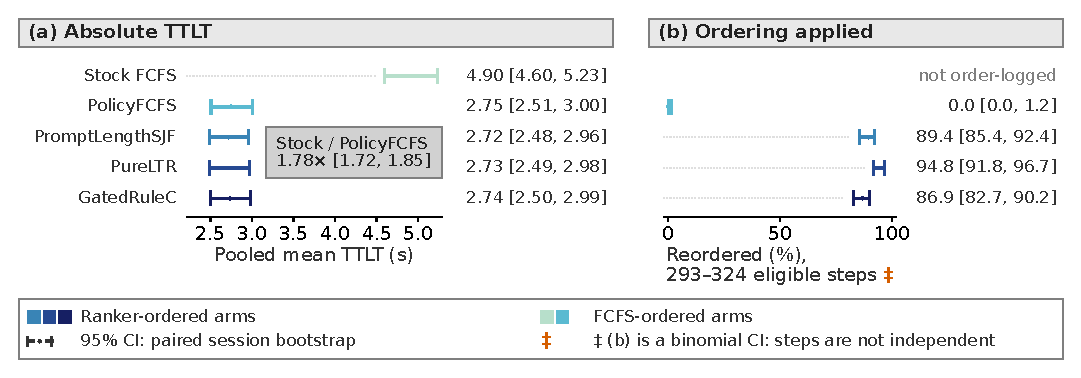
\includegraphics[width=\linewidth]{block1.pdf}
  \caption{Serving-level scheduling at the default batch cap: the
  $1.78\times$ gap between stock and \emph{PolicyFCFS} comes from the
  scheduler implementation, not from ordering, and the policies rewrote
  87--95\% of the steps that could express an order. The paired ordering
  ratios for this regime, and the 3\% margin they are judged against, are in
  Fig.~\ref{fig:regime}(a).}
  \label{fig:block1}
\end{figure*}

% Outline: Discussion (1 page cap; MUST contain 6-month future work)
\section{Discussion}

Two configured quantities decide how much of the offline schema signal
survives: the decision timeout, which forfeits 34.6\% of decisions at the
documented 15\,ms and none at 75\,ms, and the running-batch cap, which
decides whether a queue forms at all. Uncapped, ordering changed nothing; capped at 16, the learned order
beats arrival order by 4.2\% while the free length heuristic runs 8.5\%
worse than doing nothing.

\subsection{Which Gateway Optimizations Apply, and Which We Did Not Test}
Three caches are in play. \emph{Semantic response caching}, the gateway's
main lever, was unavailable: its cache excludes streaming requests, and
every captured request streamed. \emph{Prefix KV caching} is a
different mechanism that E1's byte-identical schema prefix makes plausible:
with caching on and nothing else changed, pooled mean TTLT falls by 17\% on
the two stock-scheduler arms and 22--23\% on the four policy-base arms, at a
62\% peak hit rate. That run cached the whole stream, so it did not isolate
the schema's share. E3 reports the third, schema-embedding caching,
insufficient.

A six-stage run enabled the machinery the ordering rounds disabled: the
gateway's scheduler path, queue limits and scorer discipline, at 5.76
requests/s. Mean TTLT never left the run's drift band (largest consecutive
difference 70\,ms, 1.6\% of the 4.4\,s mean,
against an ABBA drift spread of up to 1.2\%), nothing was shed, and goodput
was flat. \emph{Queue-triggered scoring} consults the scorer only when the
gateway's admission queue forms; that queue did not form at this rate, and
the decision services
recorded zero scoring requests, so the run measures trigger-path
non-activation, not a free scorer.

\subsection{What the Negative Results Buy}
Identity features fail because tool combinations essentially never repeat in
training data; removing truncation produced no detected improvement; caching
fails because a $1.9\times$
speedup does not bridge a $48\times$ budget violation. Together: neither CPU rescue makes this BERT-base Ranker fit the
15\,ms default, and fitting it needs either the GPU placement
with a recalibrated budget (75\,ms covers every decision) or a path off the
critical path, which E6 makes more valuable still.

\subsection{The Baseline Was the Result}
The one large effect in our uncontended serving measurements did not come
from our contribution. Swapping the scheduler implementation while holding
arrival order fixed cut mean time-to-last-token by 44\%; changing the order
moved it by less than the session drifted over the same hours. An earlier
round, benchmarked against the stock scheduler alone, reported uniform gains
across every policy we tried. That should have raised suspicion: policies
that order differently should not improve identically.
Those gains came from the implementation underneath. The same mistake awaits
anyone who takes a serving engine's default scheduler as a baseline; the
control must share your implementation and differ only in the variable
claimed.

\subsection{Limitations}
Offline claims rest on one workload family (ToolACE) and one label model,
the live traces come from a single agent product, and the 75 captured
payloads calibrate the synthetic workload, so they cannot double as a
validation set. The replay inherits the capture's compressed job-size
variance, which may leave ordering little room to separate.

One choice bounded the first three ordering rounds: vLLM's running-batch cap
sat at its 256-slot default. By Little's law our own
numbers put mean occupancy at roughly eleven requests in flight at
3.96\,requests/s and nineteen at 6.4, under a thirteenth of that cap. Mean
occupancy does not forbid queueing, and our logs show it did not: bursts put
11.9--12.5\% of requests behind another, but those queues drained within a
scheduling step instead of accumulating. Our calibration targeted completion
(a 95\% success criterion), not contention. E6 removes that bound and the
ordering result flips, so every ordering number here is conditional on its
regime. We did not vary how contention arises: E6 constrains the batch, while contexts large enough to
exhaust the KV cache would reach it another way.

The main matrix rests on three replay repetitions inside a single engine launch
per arm, and E6 on one cold launch per arm. The Ranker predicts decode
length
only, so prefill cost is unmodeled; the offline split is row-level; the
replay is open-loop; S2 is underpowered at $n{=}78$; and the gate's
confidence is a measured $\tau$ floor, not a calibrated probability. Serving
hardware is a vendor-modified 48\,GB RTX~4090.

\subsection{Future Work}
Six directions would occupy the next six months, in the order we would take
them. First, add an oracle-order arm sorting by measured length, separating
residual ranking error from the mechanism E6 exposes, and test whether the
gate's cost under contention can be recovered by letting abstained requests
keep a bounded slot rather than a fixed one. Second, validate
queue-triggered scoring under a load that forms the gateway queue. Third,
close the predictor-cost gap by distillation. Fourth, grow the S2 stratum to
statistical power. Fifth, move to closed-loop session benchmarks. Sixth, explore continual fine-tuning on production traffic under explicit
leakage discipline: training and evaluation traffic must never mix.

% Outline: Conclusion (exactly one paragraph)
\section{Conclusion}

Agent traffic carries a signal the serving layer currently discards: the
tool-schema text attached to every tool-bearing request. Read as text, the
request improves output-length ranking by $+0.19$ Kendall's $\tau$ over the
tuned scalar family we benchmark, and the schema itself contributes $+0.044$
of that; ranking quality changes little on the two adequately powered strata
of tool sets unseen in training (equivalence untested), where identity
features have nothing to look up. Under the gateway's documented 15\,ms decision timeout the predictor
silently loses 34.6\% of its decisions; the two CPU rescues we
pre-registered do not repair that, while a 75\,ms timeout eliminated logged
fail-open in these runs, permitting up to that much critical-path decision
latency on each scored request. Whether acting on the signal
pays depends on how contended the engine is, and that turned out to be a
configuration we set rather than a property of the traffic. With the
running-batch cap at its default the queue stayed empty at the 90th
percentile and no ordering
policy separated from another; capping the batch at sixteen put most requests
behind another, and there the learned ranker beat arrival order by 4.2\%
while ordering by prompt length ran 8.5\% slower than leaving the queue
alone. The reliability gate follows the same regime split: free when nothing
waits, and 9.5\% expensive once something does, because the requests it
declines to vouch for hold their arrival slots and block. Two levers paid in
the uncapped configuration and neither came from prediction: exchanging the stock scheduler
for the policy implementation cut mean time-to-last-token by 44\% with
arrival order held fixed, and prefix caching over the resent schemas cut a
further 17--23\%. The schema signal is real, the cheap scalar substitute for
it is worse than doing nothing, and the operator who wants either had better
check what the batch cap leaves for a scheduler to decide.

% Two rubric lines that cost nothing to honour: "Appendix A ... must be on its
% own page" and "References ... must start on a new page".
\clearpage
% Outline: Appendix A. The assignment asks for the latex_source screenshot as a
% figure and says no text is necessary, so the page is the figure plus the URL
% it evidences. The float sits at the page bottom: a two-column figure* cannot
% honour [h], and forcing it to the top puts the plate above the heading it
% belongs to.
\appendices
\section*{Appendix A: Artifact Availability}
\addcontentsline{toc}{section}{Appendix A}

\noindent
\url{https://github.com/TaliesinYang/vllm-ltr-optimization}

\begin{figure*}[!b]\centering
  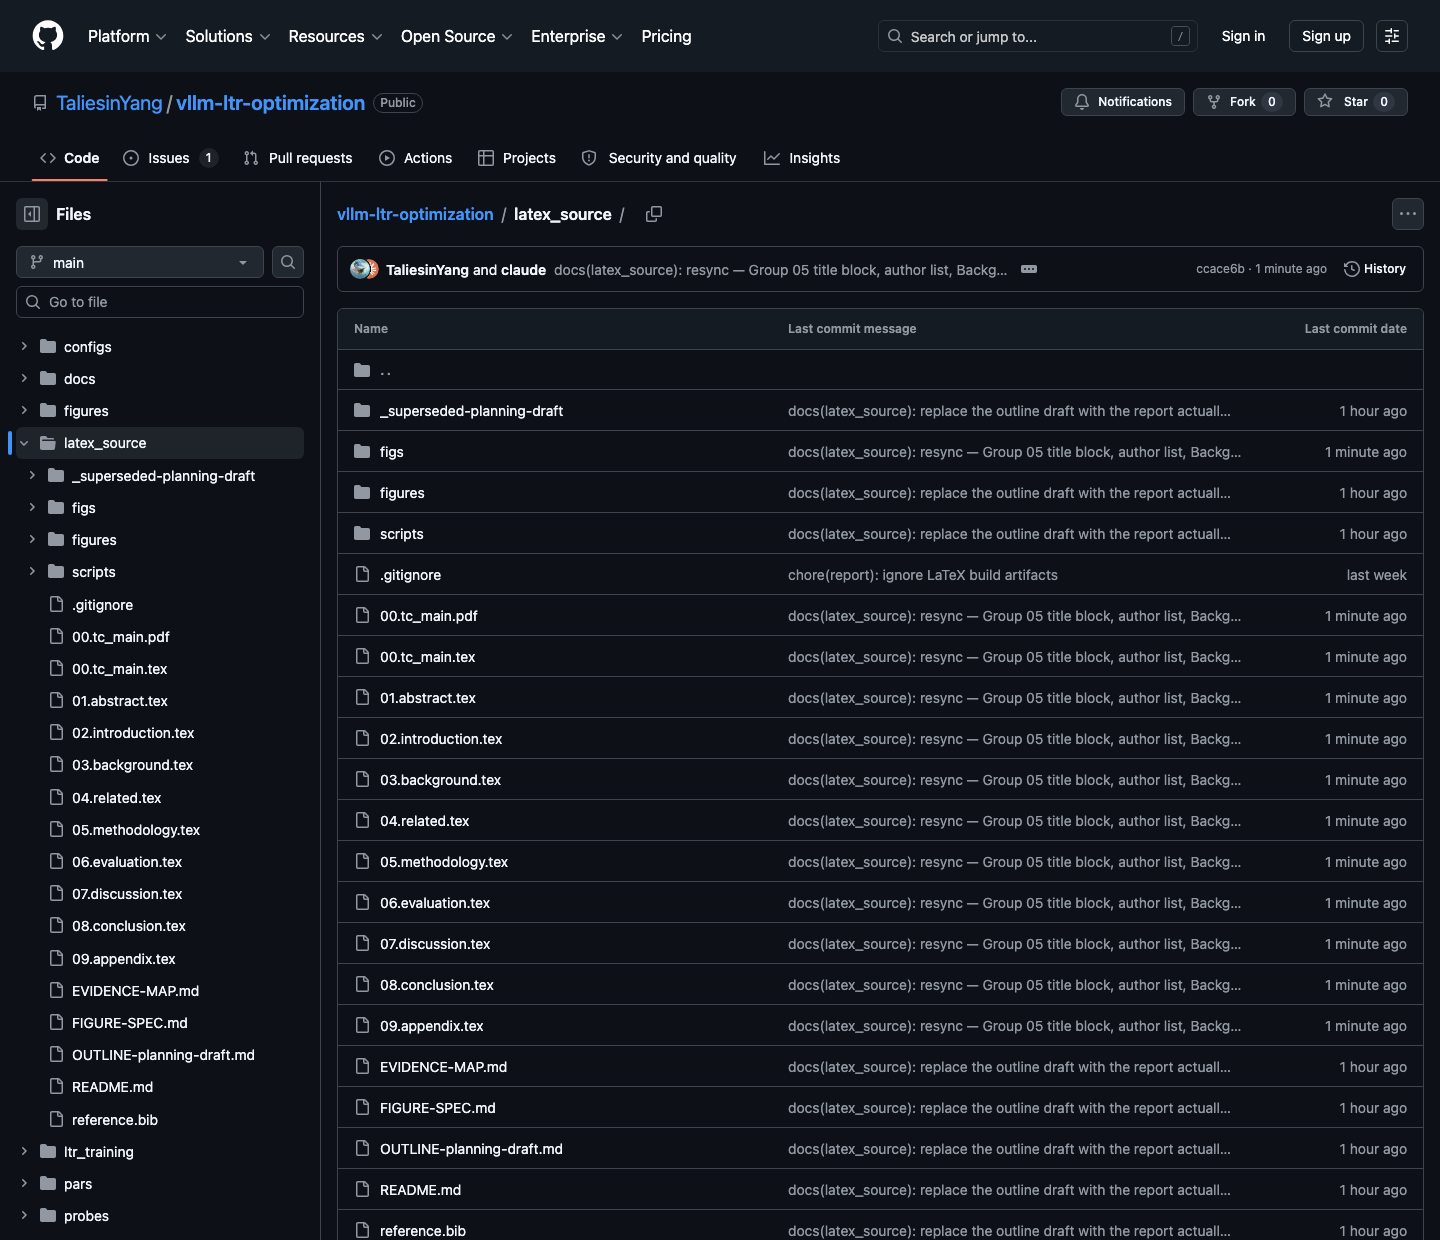
\includegraphics[width=0.92\linewidth]{latex-source-screenshot.png}
  \caption{The \texttt{latex\_source/} directory of the project repository,
  holding the LaTeX source, bibliography, figures and build checks that
  produce this report.}
  \label{fig:latexsource}
\end{figure*}

\clearpage

\bibliographystyle{IEEEtran}
\bibliography{reference}

\end{document}
